% Modeling
\section{One Dimensional Wave Equation}

In this section the one dimensional wave equation for a linear elastic material with uniform density and cross-sectional area will be derived. The derivation is based on knowledge from a number of published sources.

\begin{figure}[ht!]
\centering
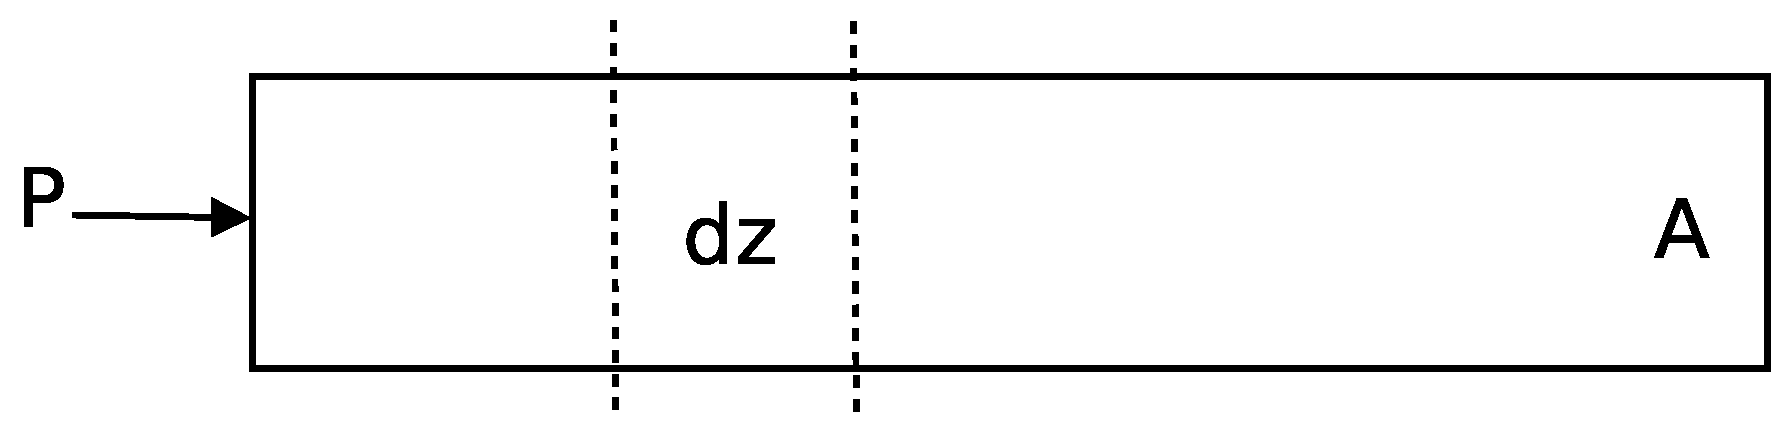
\includegraphics[width=0.8\textwidth]{eps_pics/deriveWaveRod}
\caption{Diagram for deriving the one dimensional wave equation given an axial pressure applied to one end of the material with uniform density and cross-sectional area.
	 \label{fig:deriveWaveRod}} 
\end{figure}

Figure \ref{fig:deriveWaveRod} gives a basic diagram that is used for the wave equation derivation, with $P$ being the axial pressure, $dz$ being the material's differential element of length, and $A$ being the cross-sectional area of the material. Define the stress in the z direction as:

\begin{equation}
T_3 = \frac{P}{A}
\end{equation}

\nomenclature{$P$}{Axial pressure applied to rod end}
\nomenclature{$A$}{Cross-sectional area of the rod}
\nomenclature{$dz$}{Differential element of length for the rod}
\nomenclature{$T_3$}{Stress in the z direction}

\begin{figure}[ht!]
\centering
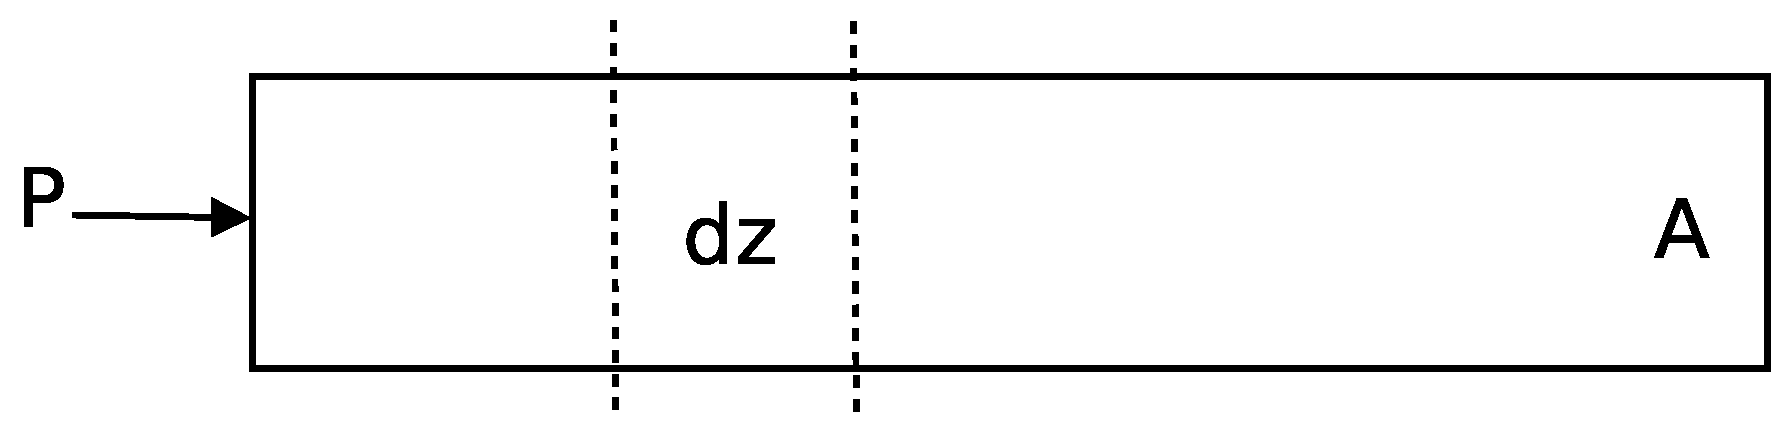
\includegraphics[width=0.8\textwidth]{eps_pics/deriveWaveRod}
\caption{Diagram for deriving the one dimensional wave equation given an axial pressure applied to one end of the material with uniform density and cross-sectional area.
	 \label{fig:deriveWaveRod}} 
\end{figure}